%% Submissions for peer-review must enable line-numbering 
%% using the lineno option in the \documentclass command.
%%
%% Preprints and camera-ready submissions do not need 
%% line numbers, and should have this option removed.
%%
%% Please note that the line numbering option requires
%% version 1.1 or newer of the wlpeerj.cls file, and
%% the corresponding author info requires v1.2

\documentclass[fleqn,10pt,lineno]{wlpeerj} % for journal submissions
% \documentclass[fleqn,10pt]{wlpeerj} % for preprint submissions

\title{Trial by phylogenetics - how model and data selection impacts the elucidation of the evolution of the Gonyaulacales (Dinophyceae).}

\author[1]{Anna Liza Kretzschmar}
\author[2]{Arjun Verma}
\author[2]{Shauna Murray}
\author[2]{Tim Kahlke}
\author[1]{Mathieu Fourment}
\author[1]{Aaron E. Darling}
\affil[1]{The ithree institute, University of Technology Sydney, Australia}
\affil[2]{c3, University of Technology Sydney, Australia}
\corrauthor[1]{Anna Liza Kretzschmar}{ anna.l.kretzschmar@gmail.com}

%\keywords{Keyword1, Keyword2, Keyword3}

\begin{abstract}
From publicly available next-gen sequencing datasets of non-model organisms, such as marine protists, arise opportunities to explore their evolutionary relationships. 
In this study we explore the effects that dataset and model selection have on the phylogenetic inference of the gonyaulacales, single celled marine algae with extensive paralogy of the phylum Dinoflagellata. 
We developed a method for identifying and extracting single copy genes from RNA-seq libraries which we used to compare phylogenies of this data set and commonly used marker genes in dinoflagellates using different phylogenetic methods.
Our results show that the exclusive use of ribosomal DNA sequences, maximum likelihood and gene concatenation were less adequate compared to a multispecies coalescence Bayesian inference approach of single copy genes for the gonyaulacales. 
This study provides an exploration of the parameter space of phylogenetic inference in species with high levels of with paralogy, and the constraints associated with this.  
\end{abstract}

\begin{document}

\flushbottom
\maketitle
\thispagestyle{empty}

%TK general comments:
% The main comment is that it needs more flow (sorry for my directness). 
%It's all in there and it's good but it often sounds more like single sentences put together than a complete text.
%LK: Aaron is smoothing the flow. Also change in the story somewhat incomming


\section*{Introduction}
Historically, availability of genetic data to infer evolutionary relationships has been a limiting factor for phylogenetics.
Now, the breadth of publicly available data sets generated by high throughput nucleotide sequencing techniques allows for an increasingly detailed investigation into the evolutionary relationships between organisms.
The quest to untangle an organsisms' phylogeny is often challenging but can inform a broad range of fields, for example epidemiology, toxicology and ecological interactions, e.g. \citep{mctavish2017and,lewis2008episodic,mutreja2011evidence,cavender2009merging,sites2011phylogenetic}.

Factors impacting phylogenetic studies range from the computational methods and availability of compute infrastructure, the methods and models applied to the data set as well data availability and the accuracy of the initial genetic data set itself.
The practitioners themselves need to have a solid understanding of the methods, including their shortcomings.
Fortunately, data availability is becoming less of a problem, due to rapid growth in public data sources and large scale projects.

An example of the breadth of publicly available data is the Marine Microbial Eukaryote Transcriptome Sequencing Project (MMETSP), which provides transcriptomes sequences of over 650 marine eukaryotic microbes \citep{keeling2014marine}. 
The MMETSP project focused on a group of understudied organisms which are abundant and play vital roles in the marine environment, from geochemical cycling, predation to symbiosis \citep{gomez2005list,gomez2012quantitative}. 
This data set offers an excellent opportunity to explore the evolutionary relationships between these taxa through phylogenetics. 

%TK I would re-write this part. It needs some flow and is not really connected to the upper parts. Something like "Another crucial factor is ... the different types of homology are Orthology, paralogy ... Orthology describes the divergence [..]. Paralogy .... and so forth
%LK: Aaron is having a go at streamlining the flow because trying to read this over and over feels like my eyeballs are bleeding
Central to phylogenetic inference is the relationship of two characters from a common ancestor, which is called homology \citep{fitch2000homology}. 
There are several types of homology, related to how the characters diverged, and determining through which mechanisms comparative traits/genes evolved is essential for choosing the correct inference model. 
Orthology is the case where the divergence of two gene copies followed a speciation event \citep{fitch1970distinguishing}. 
Paralogs are two gene copies whose divergence is preceded by gene duplication \citep{fitch1970distinguishing}.
Xenologs are gene pairs which, additional to divergence, have undergone transfer between organisms through horizontal gene transfer \citep{darby2016xenolog}.
The distinction between these cases is usually considered essential in identifying gene candidates that are informative for species evolution inference, as the selection of orthologs ensures the inclusion of a signal that is based on the speciation of the taxa examined, while selection of paralogs confounds that signal by including information that does not pertain to the speciation of the taxa \citep{du2019species}. 
As gene duplication and subsequent loss commonly occur over the course of evolution and speciation, the identification of genes that have orthologous relationships is more difficult than may seem apparent from the definition \citep{gabaldon2008large}. 
Identifying single copy genes does not ensure selection of orthologous gene copies, as the gene candidates could well be from paralogous lineages where the complimentary copy has been lost between the taxa. 
The case where paralogous homology of genes is masked by gene loss, is termed pseudoorthology \citep{koonin2005orthologs}. 

%talk about MSC addressing this scenario

Once candidate genes have been identified, there are further issues that can arise and impact the veracity of the phylogenetic inference.
Two common, well characterized types of errors are random (sampling error) and systematic errors. 
The former arises from the data, as individual gene histories may differ to the species tree. 
With a small number of genes, this error can reduce the confidence (through node support values) of the topology, and in extreme cases skew the inference away from determining a good approximation of the species tree entirely. 
Increasing the number of genes directly reduces the impact this error has on the analysis \citep{philippe2004phylogenomics,heath2008taxon}. 

Conversely, systematic errors arise due to the misspecification of the model used for the inference where an incorrect species tree topology results. 
In this case, an increase in data set size can exacerbate systematic error rather than reduce it as would happen with random errors (see Box 1). 
In the presence of this type of systematic error, the resulting inference can be positively misleading,
 with high clade support values for the incorrect tree topology, obfuscating the presence of the error \citep{jeffroy2006phylogenomics,roch2015likelihood,kubatko2007inconsistency}. 

In summary, common problems in carrying out a species tree inference arise from:\\
\begin{enumerate}[noitemsep]
\item Selection of paralogs (or pseudoorthologs). 
If genes with different evolutionary histories are selected, the gene tree will not reflect the history of either paralog and be nonsensical for species tree inference;
\item Concatenation of genes. 
Can be a statistically inconsistent estimator of the species tree due to incomplete lineage sorting (ILS) and concatenation acts as an imperfect estimator of species tree topology \citep{roch2015likelihood};
\item Inference of model adequacy from bootstrap values. 
\cite{kubatko2007inconsistency} demonstrated high bootstrap support under maximum likelihood (ML) inference for incorrect species trees with concatenated gene sets as input \citep{kubatko2007inconsistency}. 
As high bootstrap values are often used as an indicator for robust species topology resolution, this fallacy is particularly problematic if the reader/operator is unfamiliar with the statistical phenomenon.
\end{enumerate}

In this study, we explore the application of data analysis techniques which attempt to mitigate several of the pitfalls in species tree inference, beyond what has previously been applied in the study of protist phylogenetics.
The sequence data is prepared using a workflow that assembles RNA-seq data sets, identifies and extracts single copy genes across input taxa, and aligns selected genes ready for Bayesian inference (BI) phylogenetics.
Next, we evaluate the impact of model and data selection on the resulting phylogenetic inference. 
Finally, we applied the methodology to a group of organisms notorious for their extensive paralogy - the Gonyalacales (phylum: Dinoflagellata) (see box 2 for further information on the dinoflagellates).
We present a phylogenetic inference of the gonyaulacales generated under the multispecies coalescent (MSC) and compare the topology to inferences with commonly used methodologies.

\subsection*{Box 1: Statistical nomenclature \& errors this study seeks to address}
\label{sec:statbox}
For in-depth explanations see \citep{yang2014molecular}.
\begin{itemize}[noitemsep]
\item \textbf{Heterotachy:} change in evolutionary rates of sites over time, specific to lineage(s).
\item \textbf{Potential statistical error types:}
\begin{enumerate}[noitemsep]
\item random. Sampling-based error which decreases and approaches zero as the size of the data set approaches infinity.\\
\item systematic. Arises from incorrect model assumptions or problems with the model itself. 
Error type persists and increases as data set size approaches infinity. 
If strong, can override true phylogenetic signal.
\end{enumerate}
\item \textbf{Incomplete lineage sorting (ILS):} discordance of gene evolutionary history with the species evolutionary history causing the phylogenetic species tree to be misinferred. 
Difference in the topology of a gene tree compared to the species evolution can arise from the coalescence of those orthologs prior to the species divergence, where in effect the ancestral populations contain two or more already diverged copies of the gene across one or more species divergence points. 
Another mechanism is the introduction of a copy of the gene which is not based on ancestral inheritance (xenology), such as horizontal gene transfer or hybridization.
\item \textbf{Long branch attraction (LBA):} placement of two heavily divergent but distantly related sequences with each other. 
The model is unable to extract evolutionary signal due to the number of mutations that have occurred, so places the two taxa together. 
Also called the Felsenstein zone.
\end{itemize}


\subsection*{Box 2: Who/what are the Gonyaulacales?}
\label{sec:dinobox}
The gonyaulacales are an order within the super-phylum Alveolata and sub-phylum Dinoflagellata, which are an ancient eukaryotic lineage \citep{moldowan1998biogeochemical}. 
They play a role in several important ecological processes in aquatic environments where they cover a diverse array of niches such as symbionts, parasites and autotrophs. 
Some taxa can cause harmful algal blooms through proliferation (by restricting light and nutrient availability to other organisms) and/or neurotoxin production (e.g. causing paralytic shellfish poisoning, ciguatera fish poisoning) \citep{murray2016unravelling}.
Dinoflagellates possess large genomes (estimated size range 1.5 to 185 Gbp), with extensive paralogy and repetitive short sequences  \citep{casabianca2017genome}. 
In particular paralogy has proven problematic for efforts investigating the genetic content and structure of the dinoflagellates, as this feature has prevented the assembly of genomes apart from two draft genomes for \textit{Symbiodinium} which posses some of the smaller genomes \citep{shoguchi2013draft,lin2015symbiodinium}. 
Gene duplication, loss and cDNA recycling is rife within these organisms, therefore they have likely undergone complimentary gene deletion events \citep{slamovits2008widespread,murray2015gene,shoguchi2018two}. 
For a review on the genetic features of dinoflagellates see \cite{murray2016unravelling}.
While the evolutionary relationship of most orders within the dinoflagellates has been inferred with consistently high support values, one order has often escaped elucidation - the gonyaulacales. 
As neurotoxin production, which can accumulate up the food chain, is prevalent in this order, the evolution of the order is of interest to provide a frame of reference for future investigations into how the toxins have evolved \citep{shalchian2006combined,zhang2007three,saldarriaga2004molecular,hoppenrath2010dinoflagellate,murray2005improving}. 

\section*{Methods}
\subsection*{Culture conditions}
%\FloatBarrier
Cultures were isolated from locations as per Table S1 and clonal cultures established by micropipetting single cells through sterile seawater as described in in \citep{kretzschmar2017characterization}. 
Clonal cultures were maintained in 5x diluted F/2 medium \citep{holmes1991strain} and maintained at temperatures indicated in Table S1. 

\subsection*{RNA isolation, library preparation and Sequencing}
\emph{Gambierdiscus} spp. and \emph{Thecadinium} cf. \emph{kofoidii} were harvested during late exponential growth phase by filtration onto 5 $\mu$m SMWP Millipore membrane filters (Merck, DE) and washed off with sterile seawater. 
%Av just provide a range of days, eg between days 14-16 of culturing
%LK: I don't recall the exact days =/ just that it was picked to be late exponential
Cells were pelleted via centrifugation for 10 minutes at 350 rcf. 
The supernatant was decanted and 2ml of TRI Reagent (Sigma-Aldrich, subsidiary of Merck, DE) was added to the pellet and vortexed till resuspended. 
%AV life technologies 
%LK it looks like they've been bought? Or did we use Trizol reagent not Tri?
Samples were split in two and transferred to 1.5ml eppendorf tubes. 
Cellular thecae were ruptured by three rounds of freeze-thaw, with tubes transferred between liquid Nitrogen and 95 $^{\circ}$C. 
%Av specify temperature 
%LK which part? Do you mean the temperature of the liquid N2?
RNA was extracted as per the protocol for TRI Reagent \citep{rio2010purification}.
RNA eluate was purified with the RNeasy RNA clean up kit RNeasy Mini Kit (Qiagen, NL) as per protocol. 
DNA was digested with TurboDNAse (Life Technologies, subsidiary of Thermo Fischer scientific, AU). 
RNA was quantified with a Nanodrop 2000 (Thermo Scientific, Australia) and frozen at -80 $^{\circ}$C until sequencing.
The quality of samples was assessed via an Agilent 2100 Bioanalyzer at the Ramaciotti Center (UNSW, AU) and the libraries were prepared using TruSeq RNA Sample prep kit v2 (Illumina, USA). 
Paired-end sequencing was performed with a NextSeq 500 High Output run at the Ramaciotti Center (UNSW, AU) with 75bp read length for \emph{G. holmesii} and \emph{G. lapillus}; and 150bp read length for \emph{G. carpenterii}, \emph{G. polynesiensis} and \emph{T.} cf. \emph{kofoidii}.

\subsubsection*{Publicly available transcriptome libraries}
From NCBI, the \emph{Gambierdiscus excentricus} VGO790 transcriptome was downloaded under the accession ID SRR3348983 \citep{kohli2017role}, while \textit{Coolia malayensis}, \textit{Ostreopsis ovata}, \textit{Ostreopsis rhodesae} and \textit{Ostreopsis siamensis} transcriptomes were downloaded under the accession ID XXX ARJUN \citep{verma2018comparative}. 
Accession numbers available in table \ref{tbl:asmstats}. 
RNA-seq libraries for all remaining transcriptomes were generated by, and downloaded from, the Marine Microbial Eukaryote Transcriptome Sequencing Project \citep{keeling2014marine}.

\subsection*{Transcriptome processing scripts}
The workflow is separated into two parts. 
See section Implementation for script details.
\subsubsection*{Transcriptome assembly}
Individual RNA sequencing libraries are the input, which are then processed through FastQC \citep{fastqc} for quality metrics, sequences are trimmed with Trimmomatic (\texttt{LEADING:3 TRAILING:3 SLIDINGWINDOW:4:5 MINLEN:25}) \citep{bolger2014trimmomatic} and assembled with Trinity v2.4.0 (default settings for paired end libraries) \citep{haas2013novo}. 
Assemblies were then processed with BUSCOv2 with the protist specific library \citep{simao2015busco}.
%TK Are you sure that Digital normalization is there to "pool identical transcripts"? Make sure it is. My understanding is that it's to account for highly variable library sizes
%ALK my understanding is to reduce data set size: "...computational algorithm that discards redundant data and both sampling variation and the number of errors present in deep sequencing data sets. Digital normalization substantially reduces the size of data sets and accordingly decreases the memory and time requirements for de novo sequence assembly, all without significantly impacting content of the generated contigs..."
% http://ivory.idyll.org/blog/diginorm-paper-posted.html
The RNA libraries with 150bp reads generated as part of this study were also subjected to Digital Normalization \citep{diginorm} prior to assembly, to reduce data set size by removing highly similar sequences, which were then used for downstream analysis.                                                                                                                                                                                                                                                                                                                                                                                                                                                                                                                                                                                                                                                                                                                                                                                                                                                                                                                                                                                                                                                                                                                                                                                                                                                                                                                                        
\subsubsection*{Construction of multiple sequence alignments}
%TK: How did you determine if they are single copy? Just take the BUSCO genes? Or did you estimate average sequencing depth or something? Can't find it in the methods I think ...
%ALK: that's how BUSCO works, it hmmer searches sequences that should be single copy. Then reports whether they are absent, duplicated or single copy
%AD: sequencing depth methods to identify SCGs may not work very well for transcriptomes
The BUSCOv2 output from all transcriptomes from the previous step forms the input for identification of single copy genes and construction of multiple alignments. 
Any genes that BUSCOv2 identified as single copy and were present in at least 75\% of the transcriptomes were indexed, the corresponding contig extracted from the assemblies, aligned with hmmer3.1b2 \citep{eddy2015hmmer} and unaligned regions trimmed.
If several candidate sequences are processed for the same organism, a warning message in the terminal window alerts the user before proceeding. 
The output for this section was used as a basis for single copy gene phylogenetic inferences in subsequent sections.

\subsection*{Assembly analysis}
Contigs from assemblies were clustered with CD-HIT with the flags \texttt{-T 10 -M 5000 -G 0 -c 1.00 -aS 1.00 -aL 0.005} \citep{fu2012cd}. 
Protein coding regions within the clusters were predicted with Transdecoder \citep{haas2016transdecoder}. 
Amino acid clusters were clustered again with CD-HIT with the flags as previously except \texttt{-c 0.98}.
Protein sequences were analyzed with interproscan v5.27 with local lookup server \citep{quevillon2005interproscan}.

\subsection*{Phylogenetic inferences}
\subsubsection*{Ribosomal DNA based inference}
Ribosomal DNA (rDNA) sequences for the small subunit (SSU) region as well as the D1-D3 large subunit (LSU) region were acquired from NCBI \citep{coordinators2017database} and the SILVA rRNA database project \citep{silvaproj}, accession IDs in Table S3. 
Individual genes were aligned using MUSCLE \citep{edgar2004muscle} for a maximum of 8 iterations and then were concatenated in Geneious v11.3 \citep{kearse2012geneious}.
Maximum-Likelihood phylogenies were inferred using RaxML \citep{stamatakis2014raxml} with the model GTRGAMMA and with 100 bootstrap replicates.

\subsubsection*{Inference of concatenated single copy genes}
Amino acid substitution model selection was carried out with ProtTest3 with the Bayesian Information Criterion as well as the log likelihood \citep{darriba2011prottest,guindon2003simple}. 
The best-fit model for the data set identified by both criteria was VT followed by LG, however neither are available in BEAST2 so the third best model, WAG, was chosen for analysis. 
\paragraph*{Maximum likelihood with concatenated sequences.}
ML inference was run as described in the previous section, with the PROT, GAMMA and WAG flags.
\paragraph*{Bayesian inference with concatenated sequences.}
BI was run in BEAST2 with the Gamma site model with 4 discrete categories under the WAG substitution model \citep{whelan2001general}. A local random clock was used under the birth-death model 3,000,000 million chains.
\paragraph*{Bayesian probability under the MSC.}
Bayesian inference of the species tree was carried out under the *BEAST2 model in BEAST2 \citep{bouckaert2014beast}. 
The analysis was performed with the WAG amino acid substitution model \citep{whelan2001general} and with a Gamma distribution with four rate categories. 
A random local clock was employed \citep{drummond2010bayesian}. 
Posterior distributions of parameters were approximated after 300,000,000 generations of MCMC, subsampled every 5,000 generations with a burn-in of 15\%. 
The inference was run four times to evaluate convergence of parameters, then log and tree files (without burn-in) were merged. 


\subsection*{Stepping stone analysis}
%LK: Mathieu, could you update this for the new run methods used?
We estimated the marginal likelihood of the data under the coalescent (i.e. concatenated alignment) and the multispecies coalescent (*BEAST) models to compare their fitness.
We used the stepping stone algorithm by \cite{xie2011improving} along a path of 16 power posteriors.
The $\beta$ values are set equal to the quantiles of the beta distribution with shape parameter $\alpha=0.3$ and $\beta = 1$, as recommended by \cite{xie2011improving}.

\subsubsection*{Generation of figures}
Tanglegrams were generated with Dendroscope v3.5.9 \citep{huson2007dendroscope}; images were edited in GIMP \citep{gimp2008image} to improve readability.

\subsubsection*{Implementation}
The analysis work flow in section ``Transcriptome processing scripts'' was constructed as a Nextflow workflow \citep{di2017nextflow} and is available on Github at https://github.com/hydrahamster/gonya\_phylo. 
Packages within the scripts are written in bash, Python 2.7 \citep{stevens2018python} and pandas \citep{pandas}. 
Source code for the scripts is provided under an open source license.
The scripts (1) assemble RNA-seq data sets, (2) identify and extract single copy genes across input taxa with extensive paralogy, and (3) align selected genes in preparation for phylogenetic analysis.
The data sets were processed on a Genomics Virtual Lab (GVL) \citep{afgan2015genomics} instance in the NeCTAR cloud.
Phylogenetic analyses were carried out on the University of Technology Sydney's High-performance computing cluster (HPCC) and were accelerated using BEAGLE \citep{ayres2011beagle} on the GPU.
GPU processing units were either Nvidia Tesla K80 or a Tesla P100.

\section*{Results}
%TK This seems weird as the inital sentence to your results section. 
%LK: all the info is throughout the subsections, so if not here I'd have to mention zenodo in every section to make sense?
Assemblies, annotation files, BUSCOv2 output, single-copy gene alignments and single copy gene MSC BI trace files generated in this study are available on Zenodo DOI: 10.5281/zenodo.2576201

\subsection*{Transcriptomes overview}
RNA-seq libraries generated in this study are available in the NCBI sequence read archive (SRA) under the project ID SRP134273.
Sequencing of transcriptomes for \emph{Gambierdiscus} spp. and \emph{T.} cf. \emph{kofoidii} generated data sets ranging in size from 143,155,667 to 233,822,334 reads, resulting in 97,634 to 191,224 assembled contigs (table ~\ref{tbl:asmstats}). 
Clusters with gene ontology (GO) annotations made up 30.9\% to 34.8\% of the total clusters. 

%\FloatBarrier

\begin{table}[ht]
\centering
\begin{tabular}{| p{3cm} |p{2.2cm} | p{2.2cm} | p{2.2cm} | p{2.2cm} | p{2.2cm} |}

%\begin{longtable}{  | p{3cm} |p{2.2cm} | p{2.2cm} | p{2.2cm} | p{2.2cm} | p{2.2cm} |}
%\caption{\label{tbl:asmstats}Summary of transcriptome sequencing and assembly statistics.}\\
\hline
\emph{Sequences:}&\emph{G. carpenteri}&\emph{G. lapillus}&\emph{G. polynesiensis}&\emph{G. holmesii}&\emph{T.} cf. \emph{kofoidii}\\
\hline
 \multicolumn{6}{| c |}{Sequencing}\\
 \hline
\textbf{SRA accession}&SRR6821720&SRR6821722&SRR6821723&SRR6821721&SRR6821724\\
\hline
\textbf{Raw sequencing reads}&186,422,744&145,366,966&217,031,342&143,155,667&233,822,334\\
\hline
 \multicolumn{6}{| c |}{Assembly}\\
 \hline
 \textbf{Contigs \#}&105,464&148,972&114,622&191,224&97,634\\
\hline
\textbf{Average length (bp)}&607&1,139&633&953&581\\
\hline
\textbf{Maximum length (bp)}&7,448&12,370&6,608&8,198&7,922\\
\hline
  \multicolumn{6}{| c |}{Transcript clustering \& annotation}\\
\hline
\textbf{\# clusters}&139,699&92,418&139,487&107,766&116,468\\
\hline
\textbf{Contigs with GO annotations}&44,167&32,140&43,098&34,201&37,656\\ %cut -f 3 my.gff | sort | uniq | wc -l .. maybe diff to '3' but hey
\hline
\end{tabular}
\caption{\label{tbl:asmstats}Summary of transcriptome sequencing and assembly statistics.}
\end{table}

\subsection*{Single copy gene search with BUSCOv2}
Assemblies were searched with BUSCOv2 for 234 candidate single copy genes and homologs to these single copy genes were extracted. 
The single copy genes acquired though the BUSCO HMMER libraries curated for protists are reported in Table S2, as well as accession numbers and identifiers for each transcriptome. 

%TK again, describe what you did and how, then what you found.
%LK: this is the set up for the descriptions in the following sections? Trying to describe all of them at once would be confusing as hell I think. Equally re-explaining the terminology in each section doesn't seem right
\subsection*{Phylogenetic inference}
Support for branches was interpreted as follows, for ML and BI, respectively: 100\%/1.0 was considered fully supported, above 90\%/0.9 was very well supported, 80\%/0.8 and above was interpreted as relatively well supported and above 50\%/0.5 was considered weakly supported. Below 50\%/0.5 was considered unsupported.
As \emph{Azadinium spinosum}, \emph{Dinophysis acuminata} and \emph{Karenia brevis} are members of different orders (Dinophyceae ordo incertae sedis, Dinophysiales \& Gymnodiniales respectively) and are consistently placed outside of the gonyaulacales in phylogenetic analyses, their placement as an outgroup was considered a given for this study. 
Therefore, the branch separating these taxa from others was used to root ML trees in subsequent analyses where rooting was required for tree layout in visual comparisons.
\subsubsection*{rDNA based phylogeny}
%\FloatBarrier 
All nodes were supported, with a range of certainty.
The following refers to Fig. ~\ref{fig:rdna}.
Species within the genera \emph{Gambierdiscus} and \emph{Ostreopsis} resolved with their sister species with full support. 
Within the \emph{Gambierdiscus} clade, nodes are either weakly supported or fully supported. 
The two species of \emph{Alexandrium} resolve as well supported closest relatives, but do not form an individual clade. 
Deeper nodes were supported but with less certainty than the nodes near the tips. 
Two distinct clades can be observed from the topology: One including \emph{Alexandrium}, \emph{Coolia} and \emph{Ostreopsis}; another with only \emph{Gambierdiscus}. 
Sister to these clades, in descending order, was \emph{Pyrodinium}, \emph{Ceratium} and \emph{Gonaulax}, \emph{Protoceratium} and \emph{Thecadinium}. 
The outgroup was relatively well supported and included \emph{Crypthecodinium}. 
Support for deeper nodes varied from weak to well supported.

\begin{figure}[ht]
\centering
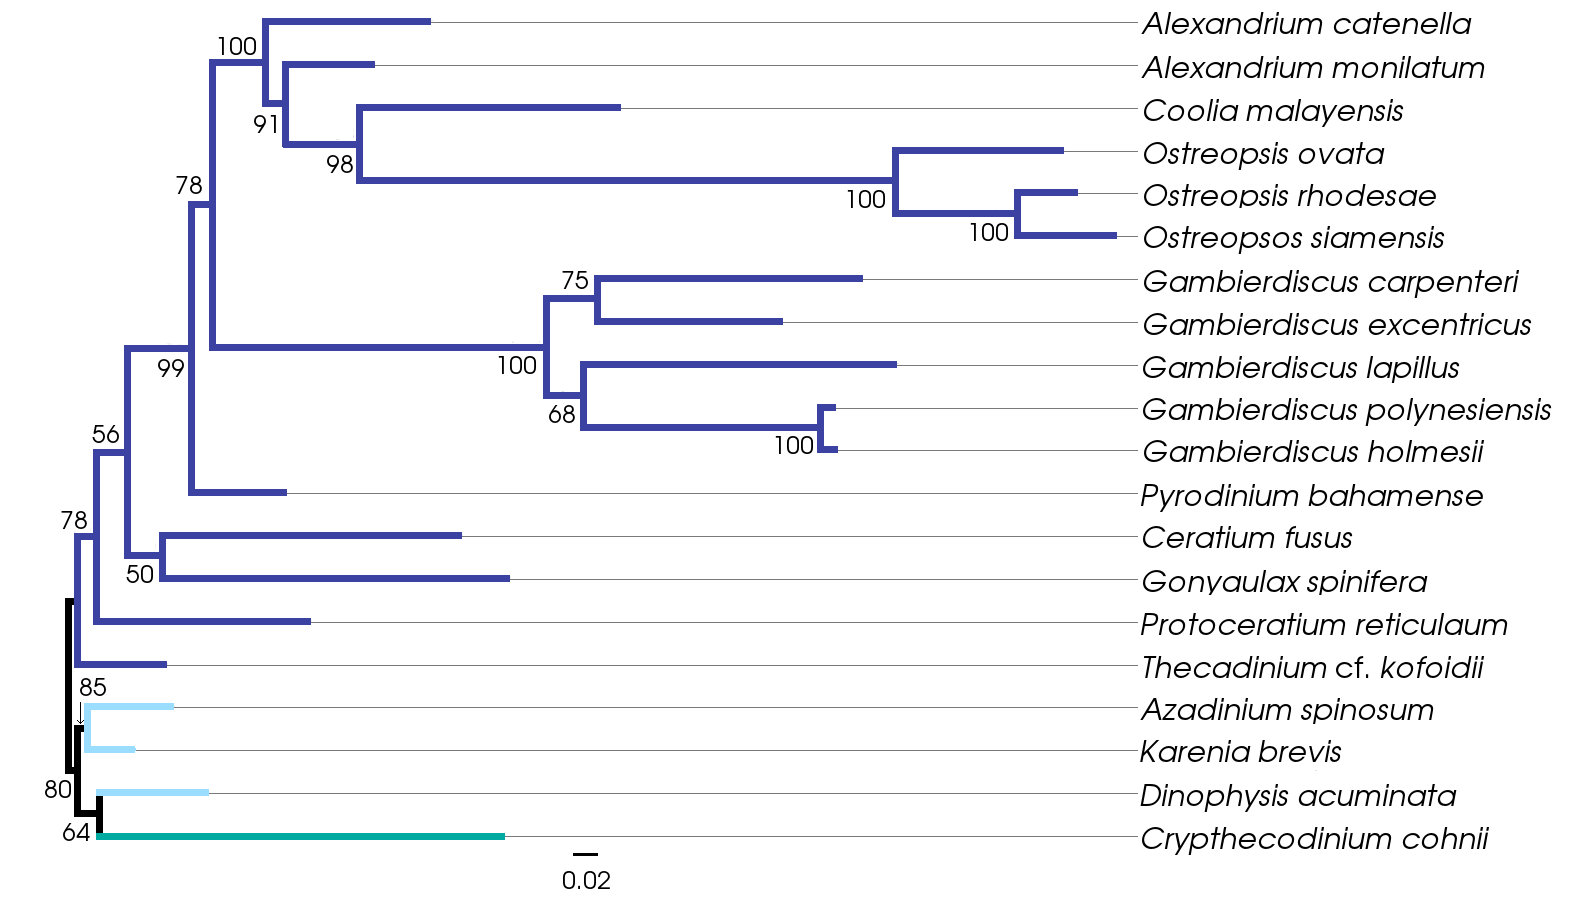
\includegraphics[width=\linewidth]{gonya-figs/rDNA-ML.png} 
\caption{Maximum likelihood phylogenetic inference of ribosomal DNA genes. Concatenation of small subunit rDNA and D1-D3 region large subunit rDNA. Accession numbers for concatenated genes in Table S3. Gonyaulacales (n=16) in purple, outgroups (n=3) in light blue and taxa \textit{incertae sedis} (n=1) in teal. Topology was rerooted on branch separating outgroup taxa with the gonyaulacales. The scale represents the expected number of substitutions per site.} 
\label{fig:rdna}
\end{figure} 
%\FloatBarrier

\subsubsection*{Concatenated single copy gene based phylogeny inferred with ML}
%\FloatBarrier
All nodes except one within the \emph{Gambierdiscus} species cluster were relatively well supported. 
Topological description in this section refers to Fig. ~\ref{fig:SCconcatML}. 
Species of the genera \emph{Alexandrium}, \emph{Gambierdiscus} and \emph{Ostreopsis} cluster as individual clades with their sister species.  
The topology shows three distinct, well supported clades: 
One encompassing \emph{Alexandrium}, \emph{Coolia} and \emph{Ostreopsis}; another which only contains \emph{Gambierdiscus}; and one which includes \emph{Pyrodinium}, \emph{Gonyaulax} and \emph{Protoceratium}. 
Sister to these clades is \emph{Thecadinium}, followed by \emph{Ceratium}.
The split of the outgroup was fully supported, while the internal nodes are very well supported. 
\emph{Crypthecodinium} was placed within the outgroup, sister to \emph{Karenia}. 
Other deeper nodes were well supported.
 
\begin{figure}[ht]
\centering
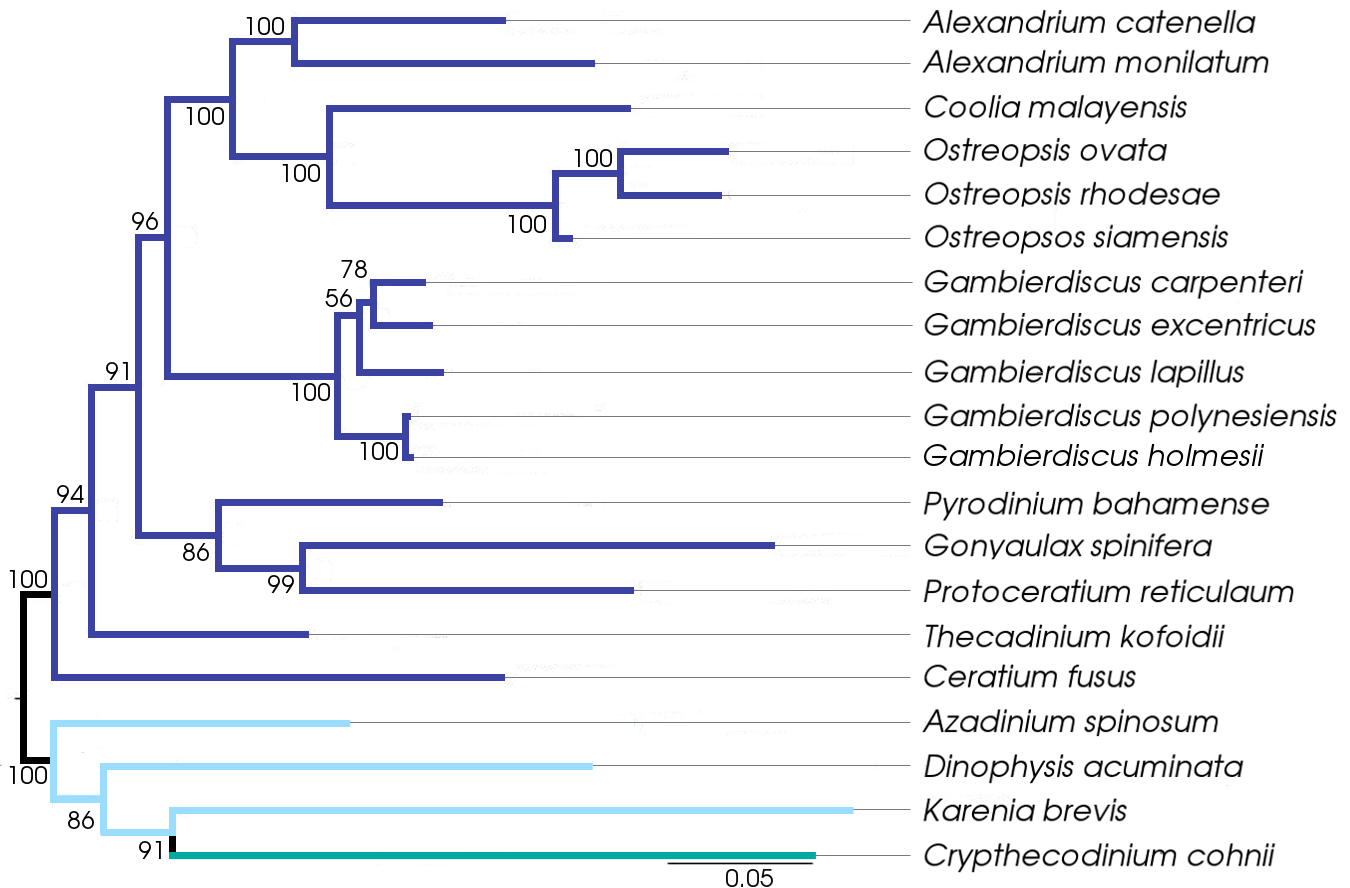
\includegraphics[width=\linewidth]{gonya-figs/SC-concat-ML-WAG.png} 
\caption{Maximum likelihood phylogenetic inference of concatenated single copy gene set (62 single copy genes from 20 taxa). Gonyaulacales (\#16) in purple, outgroups (\#3) in light blue and taxa \textit{incertae sedis} (\#1) in teal. Topology was rerooted on the branch separating the outgroup taxa from the gonyaulacales. The scale represents the expected number of substitutions per site.} 
\label{fig:SCconcatML}
\end{figure} 
%\FloatBarrier

\subsubsection*{Concatenated single copy gene based phylogeny inferred with BI}
%\FloatBarrier 
All nodes resolved with full support, except one node within the genus \textit{Gambierdiscus} which was very well supported as well as an internal node within the outgroup clade. 
The following descriptions are based on Fig. ~\ref{fig:SCconcatBI}. 
The species in the genera \textit{Alexandrium}, \textit{Gambierdiscus} and \textit{Ostreopsis} were monophyletic with full support. 
The overall topology of the gonyaulacales was resolved as three clades with \textit{Thecadinium} and then \textit{Ceratium} as ancestral lineages. 
\textit{Alexandrium}, \textit{Coolia} and \textit{Ostreopsis} clustered together, followed by \textit{Gambierdiscus} on their own in a sister clade. 
The third clade encompasses \textit{Gonyaulax}, \textit{Protoceratium} and \textit{Pyrodinium}. 

\begin{figure}[ht] 
\centering
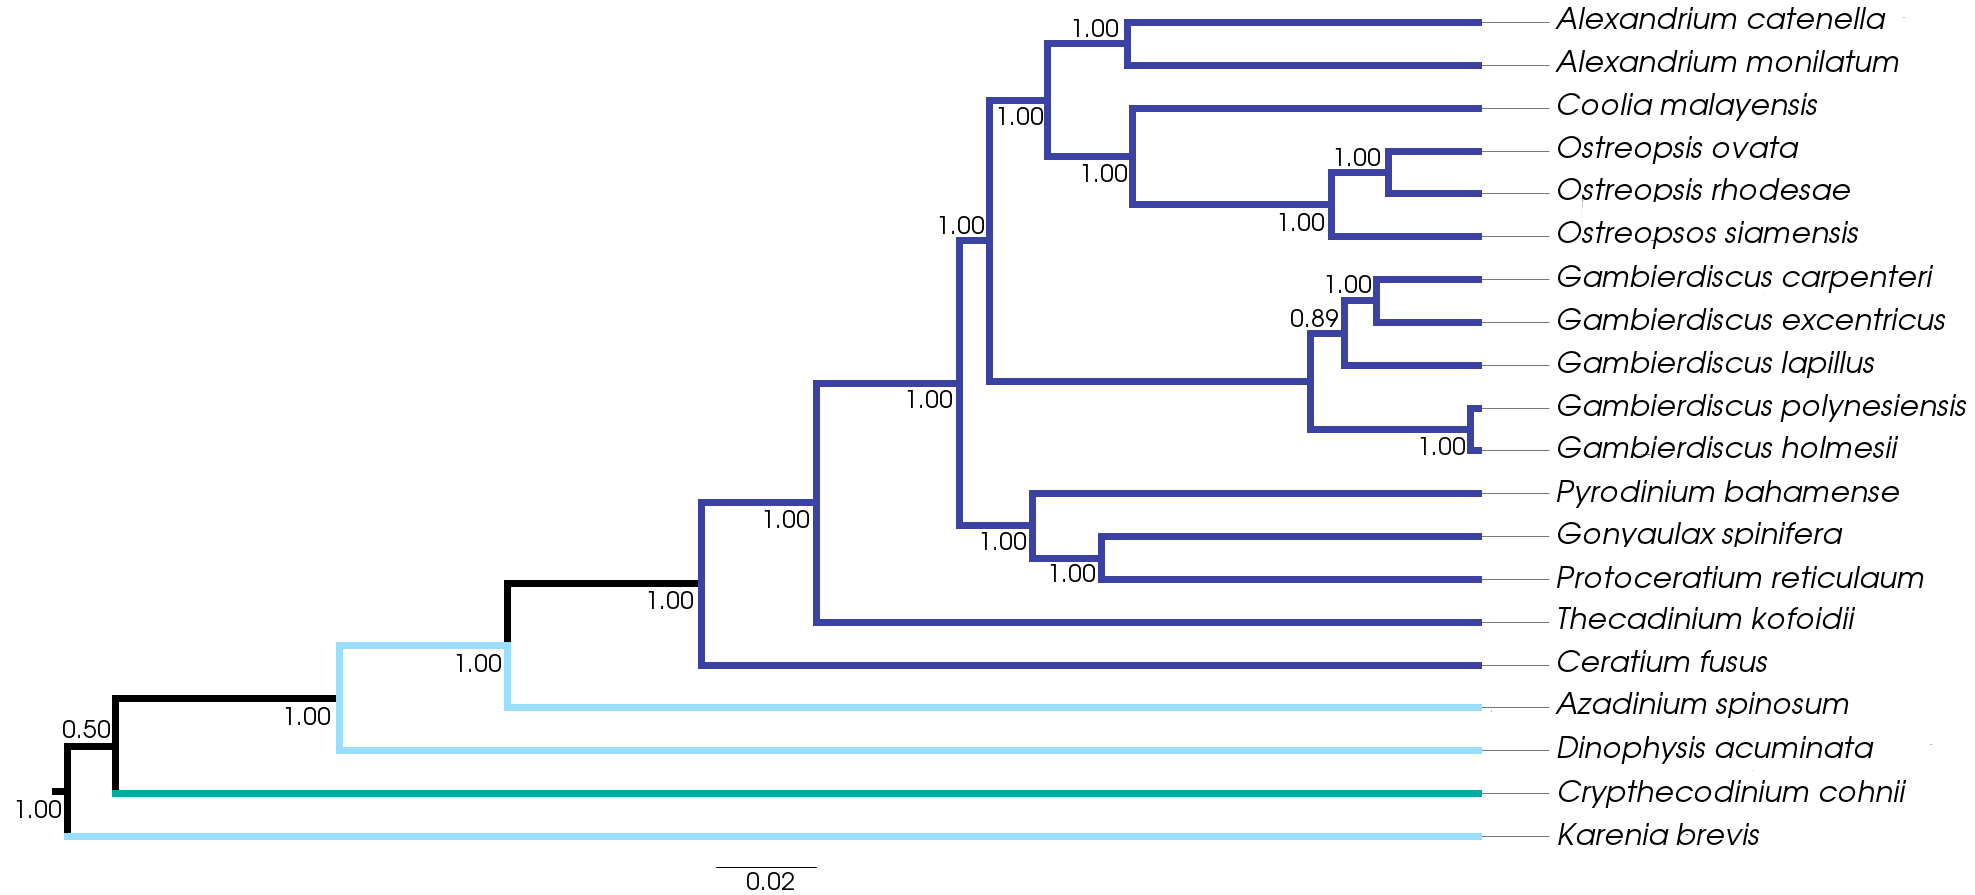
\includegraphics[width=\linewidth]{gonya-figs/SC-concat-BI.png} 
\caption{Bayesian phylogenetic inference of concatenated single copy gene set (62 single copy genes from 20 taxa). Gonyaulacales (\#16) in purple, outgroups (\#3) in light blue and taxa \textit{incertae sedis} (\#1) in teal. The scale represents the expected number of substitutions per site.} 
\label{fig:SCconcatBI}
\end{figure} 
%\FloatBarrier

\subsubsection*{Single copy gene based phylogeny under MSC}
%\FloatBarrier 
% AD: The term "resolved" is being used with what seems to be different meanings throughout this narrative and it is very confusing.
% All nodes except one within the outgroup clade resolved.
The following description is based on the topology in Fig. ~\ref{fig:SCmscBI}. 
Species of \emph{Alexandrium}, \emph{Ostreopsis} and \emph{Gambierdiscus} were either well or fully supported within their genus clades. 
The topology within the gonyaulacales resolves into three clades: 
one fully supported encompassing \emph{Alexandrium}, \emph{Coolia} and \emph{Ostreopsis};
a well supported clade with \emph{Gambierdiscus} and \emph{Pyrodinium}; 
and a weakly supported clade including \emph{Ceratium}, \emph{Gonyaulax}, \emph{Protoceratium} and \emph{Thecadinium}. 
The outgroup taxa clustered together with high support. 
\emph{Crypthecodinium} was placed as a sister taxon to the outgroup. 
Other deeper nodes were well or fully supported.

\begin{figure}[ht]
\centering
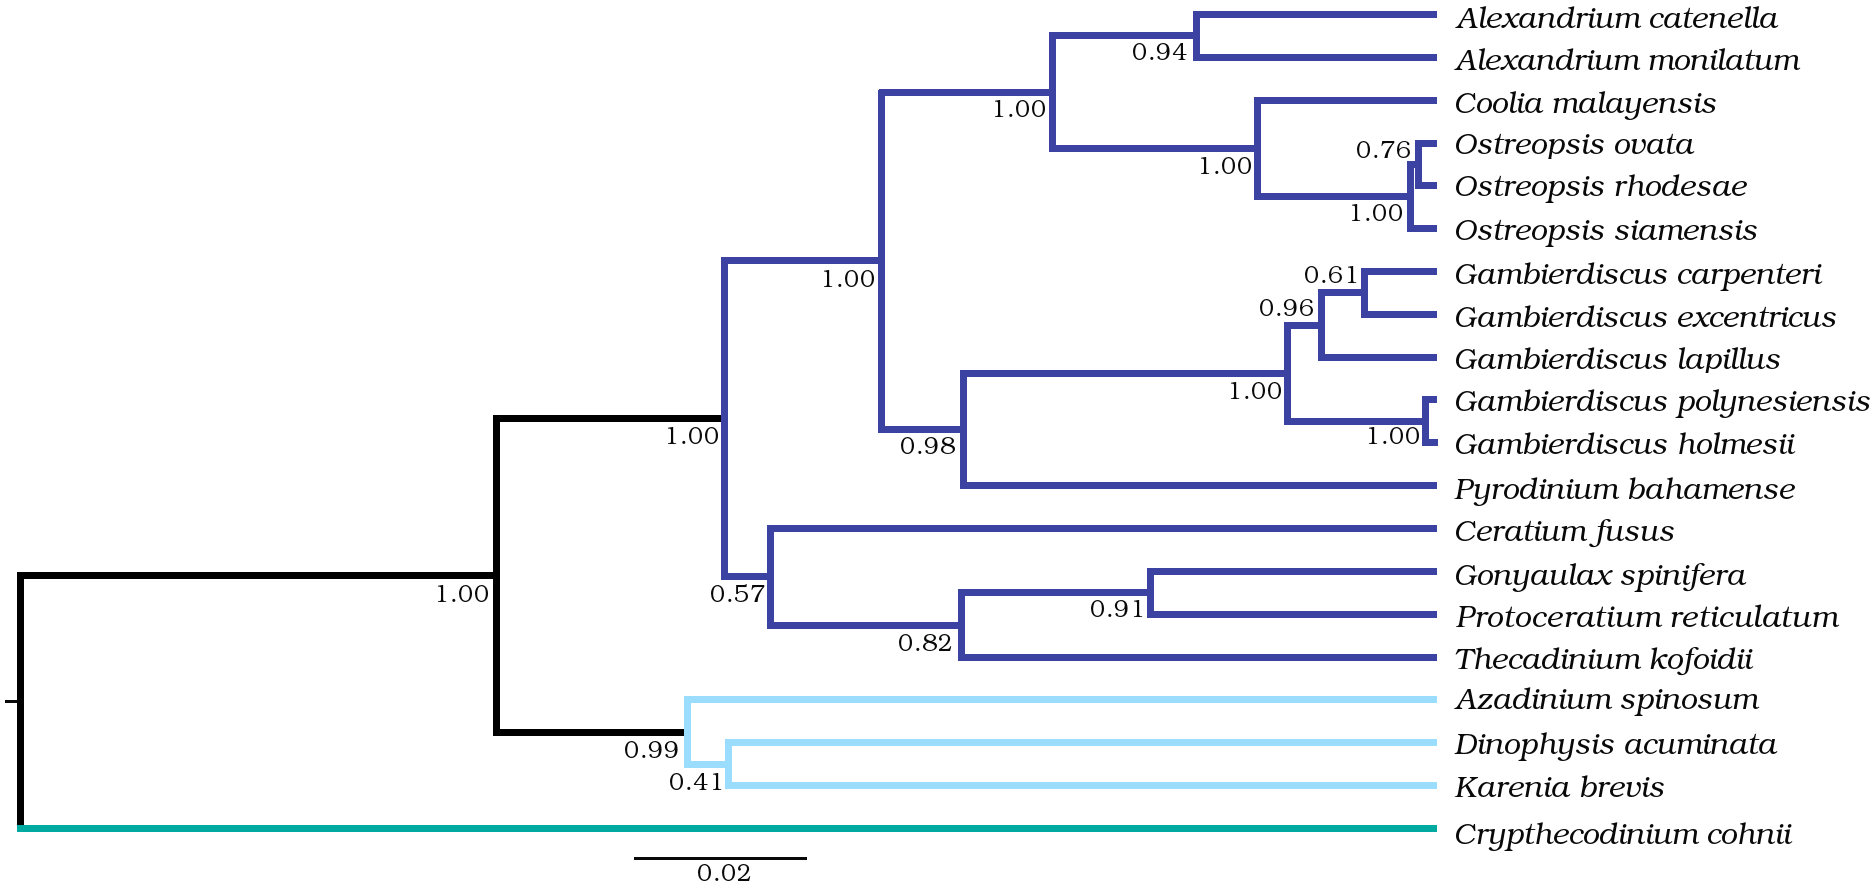
\includegraphics[width=\linewidth]{gonya-figs/Aug2-20-taxa-combined-fig-MCC-trees.png} 
\caption{Bayesian phylogenetic inference of a gonyaulacales species tree under the MSC model with 62 single copy genes from 20 taxa. Gonyaulacales (\#16) in purple, outgroups (\#3) in light blue and taxa \textit{incertae sedis} (\#1) in teal. The scale represents the expected number of substitutions per site.} 
\label{fig:SCmscBI}
\end{figure} 


\section*{Discussion}
Phylogenetic inference is a fundamental approach for exploration of the evolutionary relationships between organisms, with applications in pathology, ecology, investigating adaptive traits and many more \citep{heath2008taxon}.
Advances in sequencing technologies have seen an increase in high throughput sequencing initiatives such as MMETSP, which revealed the genomic diversity of a relatively uncharacterized group of marine microbial eukaryotes \citep{keeling2014marine}. 
%TK: ".. these .." Which?!
%It's referring directly to the sentence before, I think this should be fine?
However, the methodologies used for investigating the evolutionary relationships using this type of genome-scale data remain an obstacle, as the choice of input data and method employed influences the outcome of the inference. 
To address this, a synopsis on a method for single copy gene extraction, and synthesis of phylogenetic inference model availability and selection is presented in this study - as well as possible shortcomings of the parameters and methods selected. \\
Dinoflagellates are notorious for their large genomes with suspected whole or partial genome duplication and potential cDNA retro-insertion into the genome \citep{van2009florida,beauchemin2012dinoflagellate,slamovits2008widespread,hou2009distinct,lin2011genomic}. 
This can lead to unusually high gene copy numbers and extensive paralogy. 
With this in mind, the gonyaulacales (an order within the dinoflagellates, see box 2) presented as an ideal challenge to test the parameters of interest. 
This study presents the first species tree for the gonyaulacales with a robust method to paralogy.

The phylogenetic inference for gonyaulacales that resulted from the workflow we developed, which incorporates several of the most recent innovations in analytical methodology, resolved within-genus relationships well and shows high posterior probability support throughout the species tree (Fig. ~\ref{fig:SCmscBI}). 
The inferred species tree topology follows a broad revised taxonomic classification of the gonyaulacales based on morphological characteristics \citep{hoppenrath2017dinoflagellate} and will be used as a point of comparison to results from other commonly employed methods in later sections. 
The scripts which form the basis of this study are publicly available through github and the single copy genes used to infer the species trees, as well as the XML input and log files for the *BEAST2 runs, are available on zenodo. 
The authors hope the process presented here is transparent and reproducible for those with basic programming skills. 

\subsection*{Considerations for data set selection and pre-processing}
\subsubsection*{Quantity of taxa in phylogenetic inference}
Two concerning phenomena that can confound the veracity of conclusions drawn from phylogenetic inference are ILS and LBA. 
The risk of LBA artefacts can be reduced by denser taxon sampling to break up long branches and ensuring that the models specified are appropriate \citep{heath2008taxon}. 
The impact of ILS on phylogenetic inference has been explored through simulated data sets with a known species tree. 
While the increase in the number of genes used to infer the species phylogeny reduces the impact of ILS on the results, an increase in taxa and an even distribution thereof has been shown to have a greater impact \citep{maddison2006inferring}.
However the addition of taxa can also introduce more long branches that confound the inference \citep{heath2008taxon}. 
%Furthermore, LBA is exacerbated if ILS is present. 
%AD do you have a reference for this? I would have thought most ILS shuts off long before the sequences are so diverged that LBA on amino acid sequences becomes an issue. I mean, I can imagine it's easy to simulate situations where it happens, and I can see how it would be a problem, just not sure I believe that it's in the realm of biological possibility.
%LK: Good point, checking the references I was looking at used nt rather than AA seqs
LBA can arise if some species have disproportionately high substitution rates, leading to the presence of long and short branches in the phylogenetic tree \citep{liu2014coalescent}. %AD: note topology refers to tree without branch lengths
The gonyaulacales data set in this study includes a single representative species per genus, with the exception of \textit{Alexandrium}, \textit{Gambierdiscus} and \textit{Ostreopsis}. 
This resulted in some genera on long branches (eg. fig. ~\ref{fig:SCmscBI}: \textit{Ceratium fusus} \& \textit{Pyrodinium bahamense}) indicative of a proportionally large number of genetic changes to their closest relative.
This tree shape is consistent with sparse taxon coverage and can lead to LBA artefacts \citep{heath2008taxon}. 
To investigate the presence of ILS and as a topological comparison to the BI and ML inferences, a neighbor-joining (NJ) inference was run as well (Phylip with Protdist JTT matrix and neighbor packages \citep{felsenstein2005phylip}). 
The rationale for wanting to include this method was that NJ can recover an accurate species topology despite ILS in cases where ML would fail  \citep{mendes2017concatenation}.
However NJ is more susceptible to LBA than ML or BI methods. 
The resulting topology was so anomalous, with out and in-groups clustering together as well as negative length branch lengths, that we have chosen to exclude it from further discussion. 
Both BI and ML are more robust to the effects of LBA than NJ, where BI tends to outperform ML especially if the latter is performed conjunction with concatenation \citep{kubatko2007inconsistency,roch2015likelihood}. 
\subsubsection*{Quality of transcriptome assemblies.}
Publicly available data sets may have been generated with a variety of different methods, and their resulting quality can be highly variable, so an initial quality assessment step is essential. 
In the time since the MMETSP data sets were made available, several studies have utilized a broader range of taxa to explore evolutionary stories involving the gonyaulacales. 
However, these have relied on the assemblies supplied as part of the project. 
The stringency for quality trimming of RNA-seq libraries prior to assembly plays a role in determining the number of unique contigs recovered and the subsequent assembly quality of transcriptomes. 
Regarding the transcriptome assembly method, \cite{cohen2018mmetsp} evaluated the publicly available assemblies from MMETSP using BUSCO scores, compared to processing and re-assembly with Trinity \citep{cohen2018mmetsp}. 
\cite{cohen2018mmetsp} demonstrated that while the raw data available from the MMETSP project is an excellent resource, the assemblies available as part of the project are of a lower quality than what can be achieved with current methods \citep{cohen2018mmetsp}. 
Another factor in assembly quality is RNA-seq data processing prior to assembly, especially trimming. 
High stringency is usually favored, however \cite{macmanes2014optimal} found that this can be detrimental to the assembly and the quality cut off scores used in the present study were based on those recommendations \citep{macmanes2014optimal}.
In short, the trimming and assembly pipeline used for the assemblies available as part of MMETSP have become outdated and this is reflected in the quality comparison conducted by \cite{cohen2018mmetsp}.
To address this problem, we developed a workflow implementation of current best-practice transcriptome assembly methods as part of this study.
\paragraph*{Assembly parameters.}
Trinity was chosen as the assembler for this study based on the findings of \cite{honaas2016selecting}, in which Trinity was one of the top performing assemblers for \textit{de novo} transcriptomes as tested with \textit{Arabidopsis thaliana}. 
Further, Trinity performed well for identifying isoforms of genes and excelled at assembling highly expressed genes \citep{honaas2016selecting}.
Conversely, \cite{cerveau2016combining} found that Trinity, CLC Bio and IDBA-Tran assemblies all contain errors introduced by the assembly algorithms. 
Using a combination of all three assemblers yielded a final assembly closer to biological reality than any individual assembler, when no reference genome is available \citep{cerveau2016combining}.
As our present study uses Trinity exclusively, it may be subject to the type of errors found by \cite{cerveau2016combining} which could affect downstream analysis.
\subsubsection*{Selection of paralogs to infer species evolution.}
%\FloatBarrier
Inclusion of genes which diverged through a process other than speciation events, such as paralogs, violates the assumptions of commonly used phylogenetic models which assume all genes analysed have an orthologous relationship.
Hence the selection of orthologs, and the elimination of paralogs; or the employment of a method robust to paralogy in the dataset, is essential.
Paralogy is particularly rife in the dinoflagellates, including in the order gonyaulacales within the dinoflagellates. 
This study sought to mitigate the issues arising from paralog comparison by isolating single copy genes, using the curated BUSCO gene collection and software to facilitate the process. 
As BUSCO uses lineage specific profile HMM libraries designed to target single copy genes, and the output distinguishes between single copy genes and duplications, it presents a method for reliably screening for single copy genes for phylogenomics \citep{waterhouse2017busco}.
Only one other study by \cite{price2017robust} sought to address the issue of paralogy for species inference within the dinoflagellates, by selecting single genes as input. 
However there are several issues with the study presented by \cite{price2017robust}. 
First, the assemblies used are from the MMETSP project, which employed outdated assembly methods as mentioned previously, and hence could present single copy genes which are instead hybrids of paralogs. 
%LK: Aaron, did we settle on keeping this sentence in? I remember there being some contention about the hybrids thing
Further, the methodology for identifying and selecting the single copy genes was not described in the publication and is not available upon request from the authors. 
Correspondence with the author of that study established that there was no documentation for the commands that the authors executed, so no record of how the genes were attained was available. 
Hence it was impossible to compare the parameters that went into identification of single copy genes and it was not possible to scrutinize or reproduce the study.
Lastly, in that study the genes were concatenated and the evolutionary relationships were inferred using ML. 
While the node bootstrap values are high, that could be due to systematic error as outlined in previous sections.
Critically, this methodology is susceptible to pseudoorthology selection.
The difference in tree topology inferred by \cite{price2017robust} and by our study lies in the organization of sister taxa (Fig. ~\ref{fig:tanglePrice}). 
The \cite{price2017robust} study placed \emph{Alexandrium} spp. as the closest genus to \emph{Gambierdiscus}, while this study places \emph{Pyrodinium} as sister. 
As some \emph{Gambierdiscus} spp. produce polyketide toxins which cause ciguatera fish poisoning, establishing the close relations to \emph{Gambierdiscus} is important for investigating the toxin evolution \citep{pawlowiez2014transcriptome}.
The placement of the genus \emph{Azadinium} is also a point of difference, as \cite{price2017robust} place it as part of the gonyaulacales, while this study firmly places this genus as an outgroup with \emph{Dinophysis} spp. and \emph{Karenia} spp.
As \emph{Azadinium} spp. also produce polyketide toxins that cause azaspiracid shellfish poisoning, their placement is important for investigating polyketide toxin evolution \citep{meyer2015transcriptomic}.
 
\begin{figure}[ht]
\centering
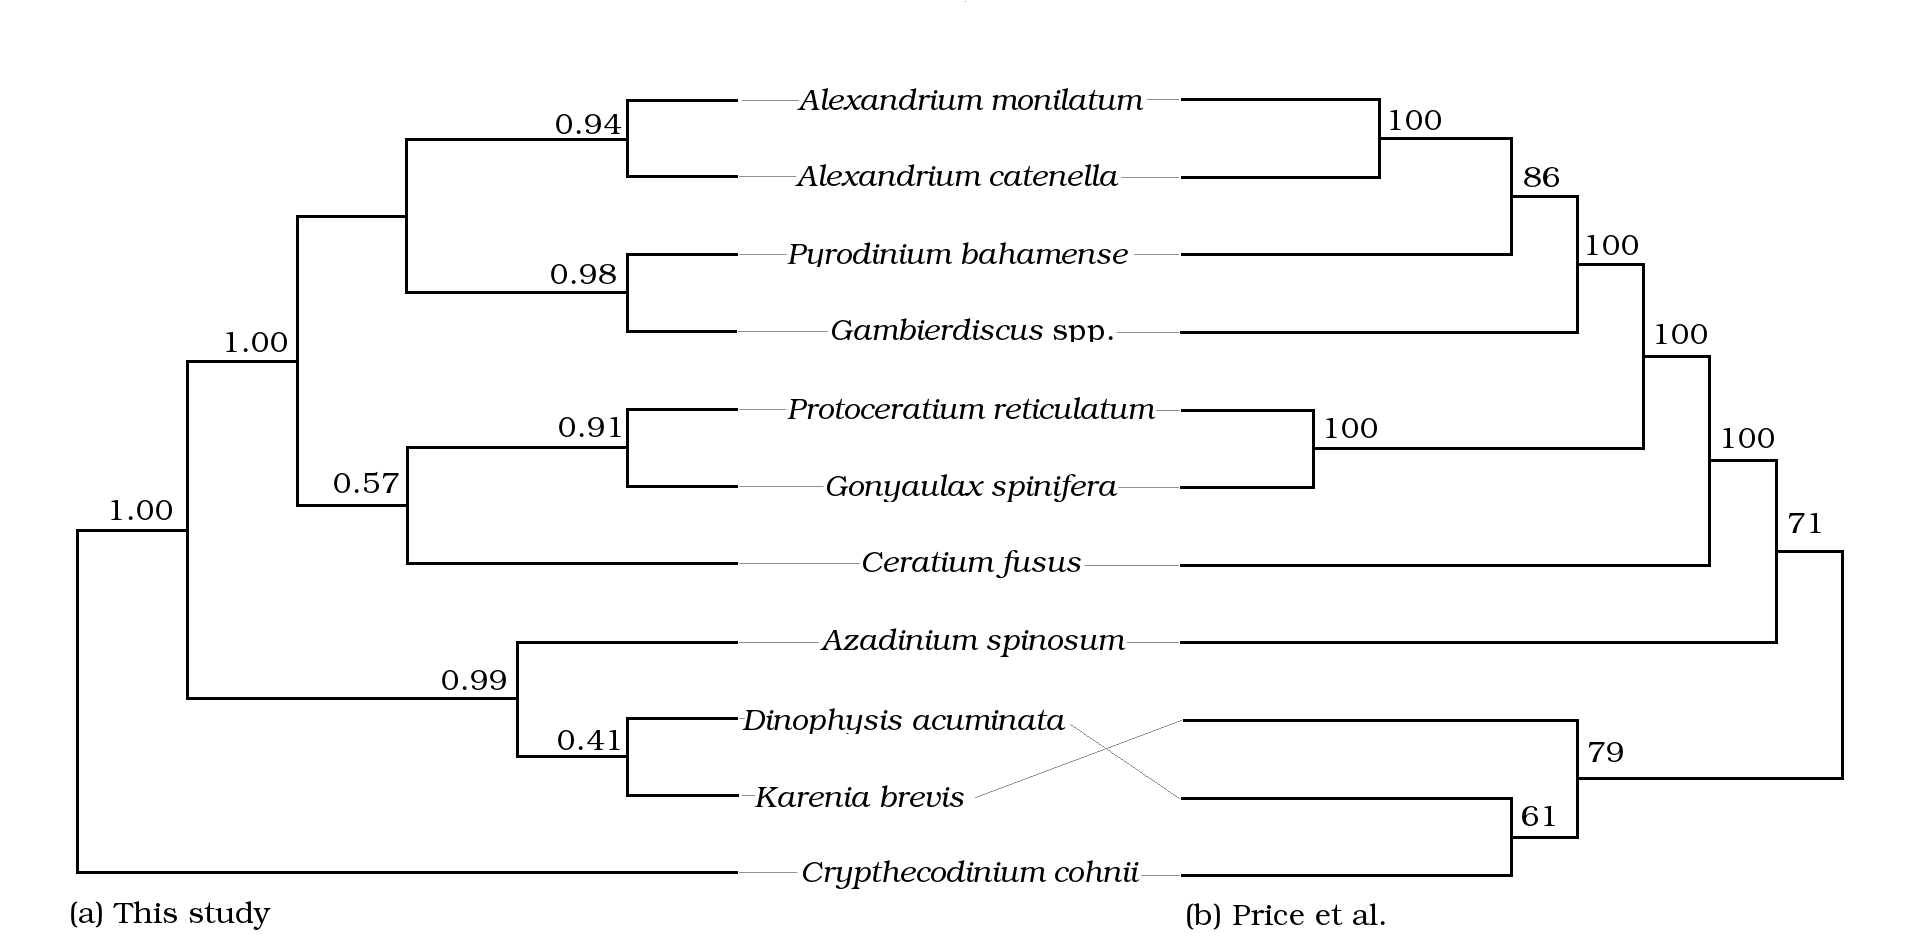
\includegraphics[width=\linewidth]{gonya-figs/Price-comparison.png}
\caption{Tanglegram of the single copy gene topologies presented in (a) this study under MSC; and (b) concatenated by \cite{price2017robust}. Taxa not common to either study are not shown due to the reduced topologies from the original studies, closest PP or BS to branch split were included.} 
\label{fig:tanglePrice}
\end{figure} 
%\FloatBarrier
\subsubsection*{Model selection for inference.} The issue of model choice is an important one, as the choice of model can heavily influence the resulting topology. 
Mis-specification of the model, or individual parameters, can lead to a well supported but erroneous result. 
While models are a simplistic approximation of the underlying biological drivers of evolutionary processes, getting as close an approximation as possible is essential \citep{box1979all}. 
However under- and over-parameterization have been shown to impact topology and PPs to varying degrees, in and outside the Felsenstein zone \citep{lemmon2004importance}. 
Stepping stone sampling compares the marginal likelihood of both the prior and the posterior of a model, while penalizing for overparameterization and can be used to compare the fit of one model compared to another for a given data set \citep{xie2010improving}. 
To compare how well concatenation vs. MSC fits the single copy gene data set used in this study, stepping stone comparison was conducted.

\subsection*{Comparison to commonly employed models and data sets}
\subsubsection*{Phylogenetic inference using ribosomal genes.}
%\FloatBarrier 
Using LSU or SSU rDNA regions for phylogenetics is common practice, at times supplemented with a small number of other genes \citep{shalchian2006combined,zhang2007three,saldarriaga2004molecular,murray2005improving,hoppenrath2010dinoflagellate}. 
It is important to acknowledge that these represent the evolutionary history of highly conserved genes, which does not necessarily represent the species evolution and assumptions of their congruence is statistically inadequate \citep{degnan2009gene}.
Utilization of rDNA loci made sense when study designs were bound by sequencing and computational limitations, as they were a universally available proxy which was informative. 
Due to this legacy they continue to be commonly employed, exclusively or as part of a subset of genes for analysis, for the gonyaulacales. 
%MF the 2 topologies seem different in tanglerDNA but lines joining taxa do not cross. Am I missing something
Comparing the topology from a rDNA ML inference with the single gene copy MSC phylogeny presented here (Fig. ~\ref{fig:tanglerDNA}) shows that most clades in both topologies were completely or very well supported. 
Within the genera \emph{Gambierdiscus} and \emph{Ostreopsis}, the species resolution differed between the two data sets. 
In several cases, the placement of sister taxa was incongruous between the two analyses. 
For example, the rDNA concatenation data set places \emph{Ceratium} \& \emph{Gonyaulax} as well as \emph{Alexandrium} and \emph{Gambierdiscus} as sister taxa, while the single copy gene data set under MSC places \emph{Gonyaulax} with \emph{Protoceratium} and \emph{Gambierdiscus} with \emph{Pyrodinium}. 
This is an example of how using rDNA segments as a proxy for species evolution produces different results than an analysis of single-copy protein coding genes.

\begin{figure}[ht]
\centering
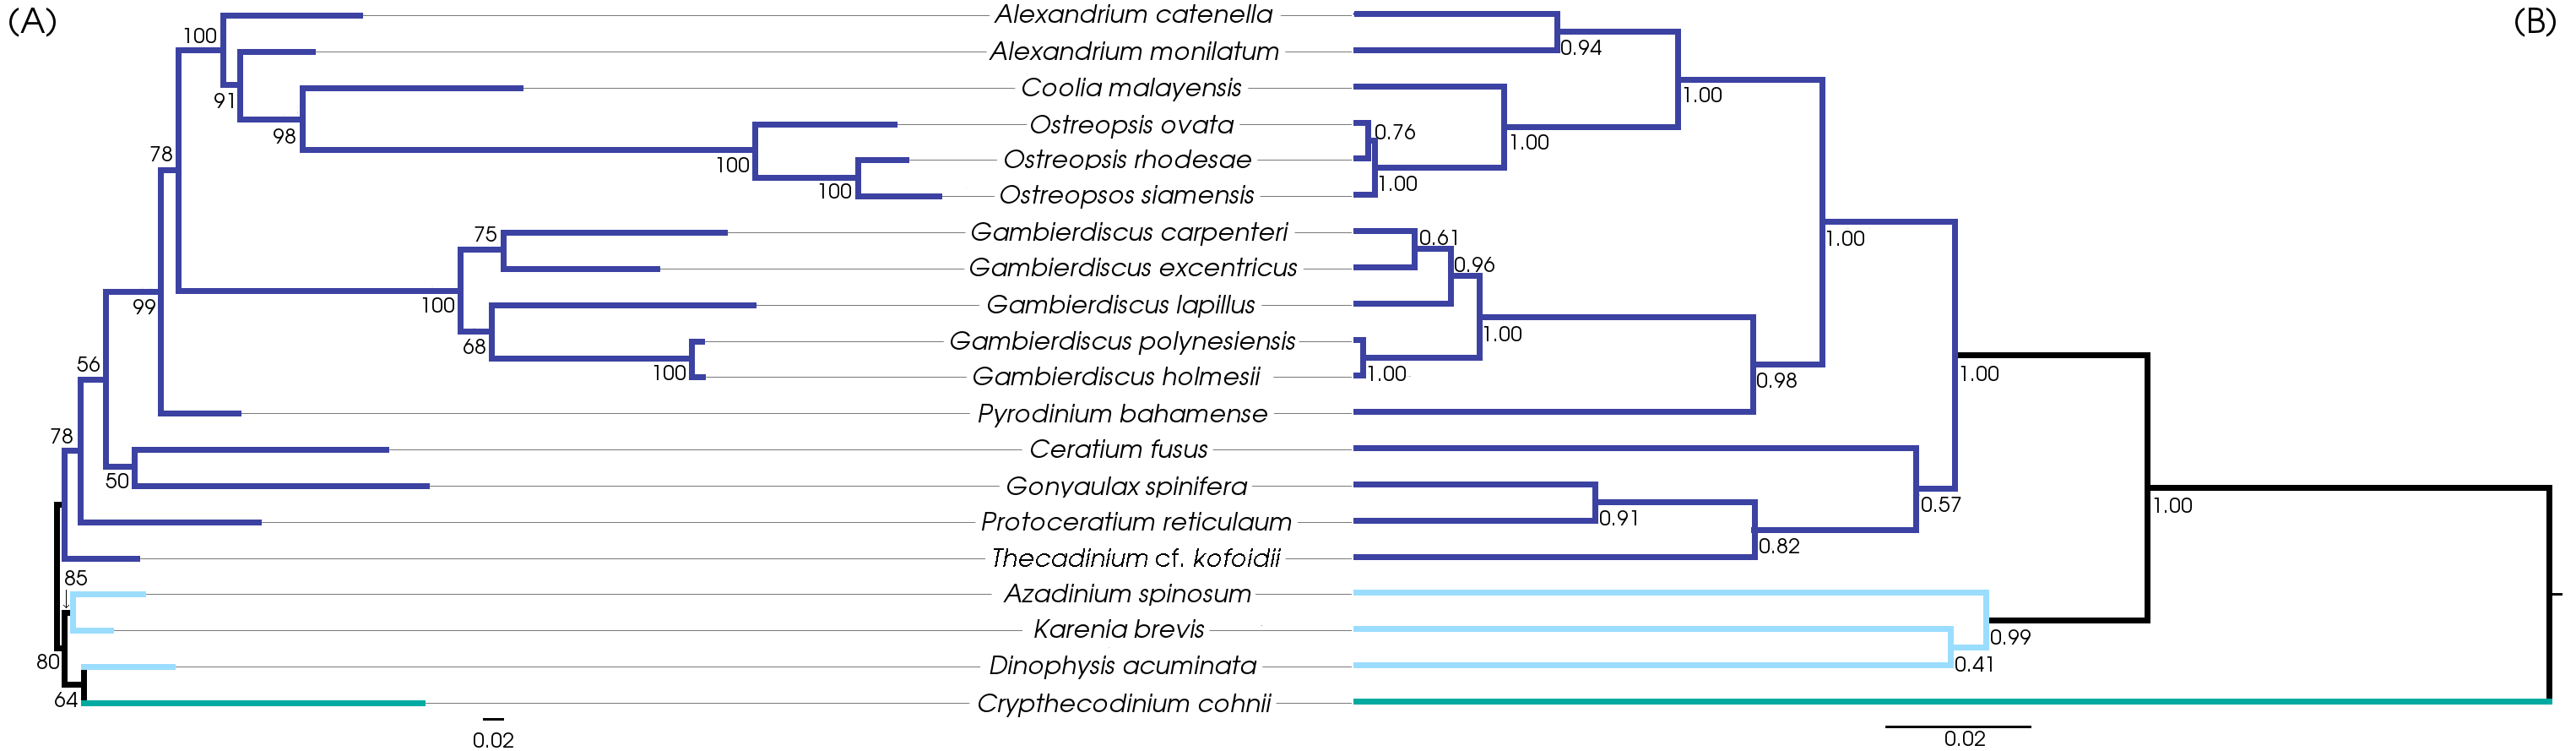
\includegraphics[width=\linewidth]{gonya-figs/MSC-BI-vs-rDNA-ML.png} 
\caption{Tanglegram showing the topological differences in phylogenies from (A) concatenated rDNA genes (SSU and D1-D3 LSU) inferred with ML; and (B) MSC inference with 58 single copy genes. Gonyaulacales (\#16) in purple, outgroups (\#3) in light blue and taxa \textit{incertae sedis} (\#1) in teal.} 
\label{fig:tanglerDNA}
\end{figure} 
%\FloatBarrier


\subsubsection*{Concatenating selected genes and using ML methods for species inference.}
%\FloatBarrier
Concatenation of alignments coupled with ML inference is a commonly used method as it is less computationally demanding than BI methods. 
However as demonstrated by \cite{kubatko2007inconsistency} and \cite{roch2015likelihood}, this approach is error prone. 
Concatenation assumes uniform evolutionary history across genes, with a small amount of variation possible - however this still averages the evolutionary rate for all the input genes which doesn't allow for drastically divergent gene histories \citep{roch2015likelihood}. 
The combination of concatenation and ML for phylogentic inference can result in high bootstrap values for incorrectly resolved clades, over inflating confidence in erroneous topologies \citep{degnan2009gene}. 
The application of concatenation in combination with ML is common practice in phylogenetic studies for gonyaulacoids  \citep{shalchian2006combined,zhang2007three,saldarriaga2004molecular,murray2005improving,hoppenrath2010dinoflagellate}.
We investigated whether use of a technique explicitly designed to handle multiple genes to estimate species trees would yield different results than concatenation and ML. 
A comparison between a BI inference under MSC compared to concatenated ML inference on the same single copy gene data set shows differences in topology (Fig. ~\ref{fig:tangleconcatML}). 
The species resolution within the genera \emph{Alexandrium}, \emph{Gambierdiscus} and \emph{Ostreopsis} matches between the two inference methods. 
The major difference is of the \emph{Pyrodinium} placement, where the BI MSC approach places the genus sister to \emph{Gambierdiscus} while the concatenated ML approach places it with \emph{Gonyaulax} and \emph{Protoceratium}. 
Further, the deeper branches of the phylogenies differ. 
The BI MSC method clusters \emph{Ceratium}, \emph{Gonyaulax}, \emph{Protoceratium} and \emph{Thecadinium} as a clade, while the concatenated ML approach clusters \emph{Gonyaulax}, \emph{Protoceratium} and \emph{Pyrodinium} as a clade to which \emph{Thecadinium} and then \emph{Ceratium} feature as ancestral genera. 

\begin{figure}[ht]
\centering
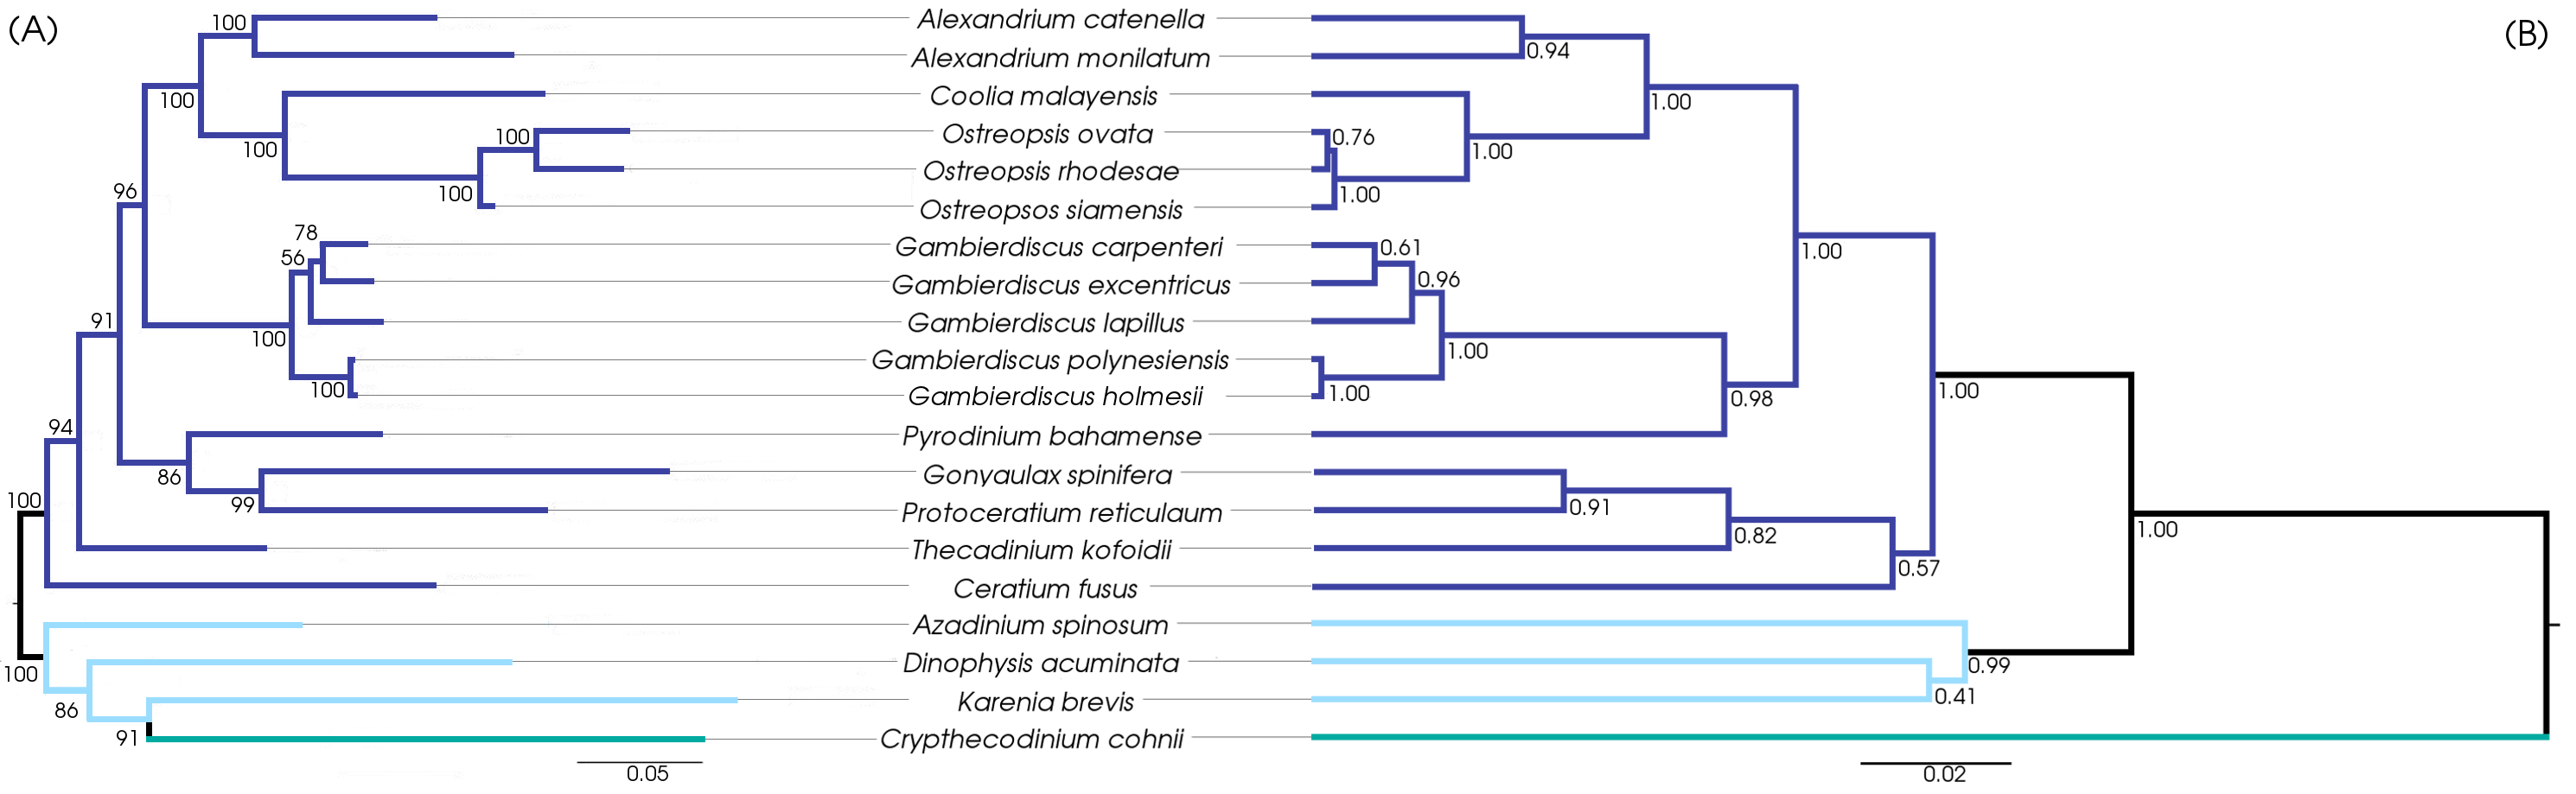
\includegraphics[width=\linewidth]{gonya-figs/MSC-BI-vs-singlecopy-concat-ML.png} 
\caption{Tanglegram showing the topological differences in phylogenies with same 58 single copy gene alignments as input. (A) concatenated ML inference; and (B) MSC *BEAST2 inference. Gonyaulacales (\#16) in purple, outgroups (\#3) in light blue and taxa \textit{incertae sedis} (\#1) in teal.} 
\label{fig:tangleconcatML}
\end{figure} 
%\FloatBarrier

\subsubsection*{Concatenating selected genes and using BI methods for species inference.}
%\FloatBarrier
Even within a BI framework concatenation can introduce a number of errors. 
Under simulated data sets, even under the coalescent methods, the species tree topology is inaccurate when concatenation is used \citep{kubatko2007inconsistency}. 
Further to that, the PP values tend to be overestimated for concatenation \citep{suzuki2002overcredibility}. 
Theoretically for the gonyaulacales, and taxa prone to paralogy and convoluted evolutionary histories, the MSC is a preferable approach to concatenation as MSC is more robust to ILS \& LBA artifacts as well as pseudoorthologs \citep{liu2014coalescent,du2019species}. 
To isolate the effects of phylogenetic model from those of the statistical framework (ML vs BI), the single copy gene data set was run with BI both under MSC and with concatenation (Fig. ~\ref{fig:tangleconcatBI}). 
We then used a statistical framework to compare the two model approaches to verify the veracity of model adequacy through stepping stone sampling. 
%LK: Mathieu, could you update this for the new run methods used?
PATH sampling is an adequate method for objectively comparing the model parameters for relaxed clock models while penalizing for over-parameterization \citep{baele2012accurate}. 
The marginal likelihoods for the concatenated single copy gene dataset compared to under MSC was over 10,000 log units higher, favoring the MSC approach significantly. 
The drastic difference in marginal likelihood between the models could be due to the likely inclusion of pseudoorthologs in the dataset, a phenomenon that MSC is robust to, unlike concatenation \citep{du2019species,roch2015likelihood}.
However stepping stone methods are sensitive to the number of steps employed in the analysis, which should be taken under consideration when interpreting these results. \\
The resolution of \textit{Alexandrium}, \textit{Coolia} and \textit{Ostreopsis} was identical between the two methods. 
Further, the species resolution within the genera \textit{Gambierdiscus} and \textit{Ostreopsis} was also identical. 
Differences were found in the topology, in that \textit{Pyrodinium} clustered with \textit{Gambierdiscus} in the MSC analysis, while for concatenation this genus clusters with \textit{Gonyalax} and \textit{Protoceratium}. 
The \textit{Pyrodinium} placement also differs to the study by \cite{price2017robust} (Fig. ~\ref{fig:tanglePrice}), where the genus is more closely related to \textit{Alexandrium} rather than \textit{Gonyaulax} and \textit{Protoceratium} in the BI topology. 
Further, in the MSC analysis \textit{Ceratium}, \textit{Gonyalax}, \textit{Protoceratium} and \textit{Thecadinium} form their own clade while with concatenation, \textit{Ceratium} and \textit{Thecadinium} are ancestral genera to the rest of the gonyaulacales. 
There is a marked difference in the internal branch arrangement, resulting in different taxa clustering, between the concatenation and MSC methods.
The concatenated approach closely mirrors the ML arrangement of taxa, apart from \textit{Crypthecodinium} placement. 
The main difference between the ML and BI concatenated inferences is the predicted number of protein changes along the branches and both inferences are topologically distinct to the MSC approach.

\begin{figure}[ht]
\centering
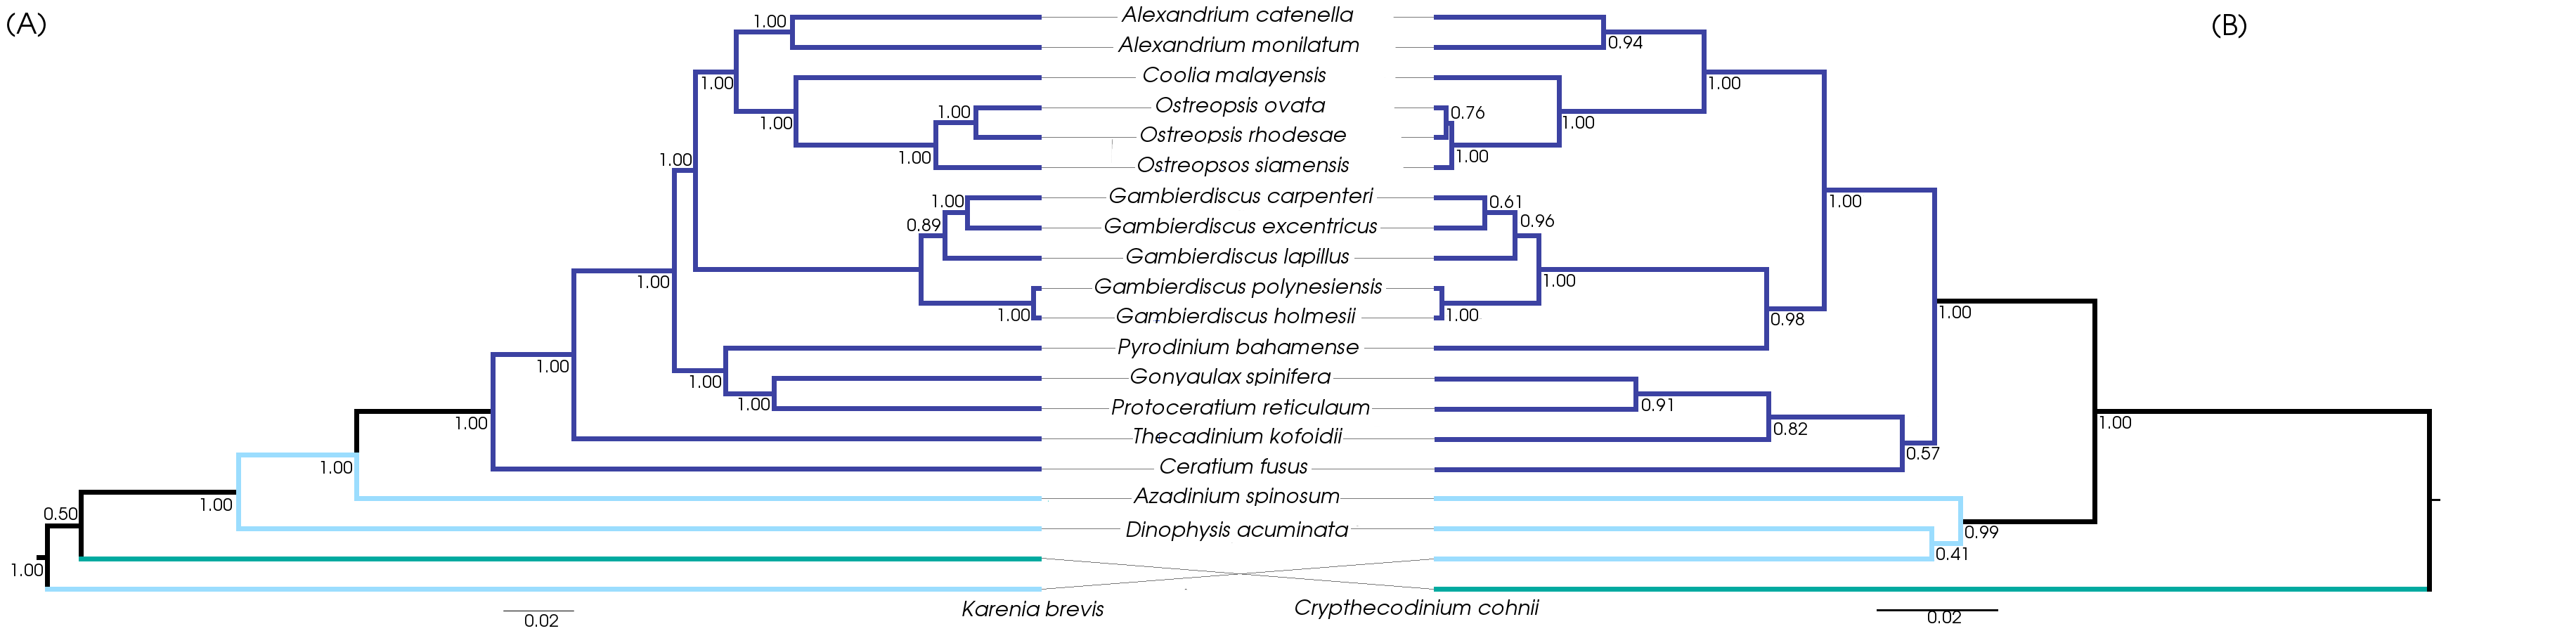
\includegraphics[width=\linewidth]{gonya-figs/SC-MSC-BI-vs-SC-concat-BI.png} 
\caption{Tanglegram showing the topological differences in phylogenies with same 58 single copy gene alignments as input. (A) concatenated BEAST2; and (B) MSC *BEAST2 inference. Gonyaulacales (\#16) in purple, outgroups (\#3) in light blue and taxa \textit{incertae sedis} (\#1) in teal.} 
\label{fig:tangleconcatBI}
\end{figure} 
%\FloatBarrier



\subsection*{Areas for possible improvement of this study}
In the previous section we identified potential problems with common approaches to species inference in the literature, and in particular for the gonyaulacales. 
We then sought to evaluate the effects of different methodological approaches on analytical results in the gonyaulacales. 
There are several important limitations to our study. 
\paragraph*{Contamination of other taxa.} 
The 650+ RNA extract submission to MMETSP was from a large number of investigators and low level contamination is inherent in the project's data set \citep{keeling2014marine}. 
As the cultures tested in all the studies contributing to this data set were not axenic, contamination could be bacterial or eukaryotic in nature. 
While any contaminating bacterial genes in our data would likely be heavily diverged and therefore obvious, eukaryotic contamination may be more subtle.
\paragraph*{No representative genome for comparison.} 
Without an available reference genome, it is difficult to evaluate the accuracy of the transcriptome assembly and whether the genes selected are single copies, or misassemblies of paralogs.
\paragraph*{Different methods for RNA-seq.} 
Three different approaches for RNA-seq library generation were employed for the libraries used in this study, the MMETSP taxa were sequences on HiSeq platform with 50nt reads; while all other taxa were sequenced on the NextSeq platform with 75nt or 150nt reads. 
The different sequencing methods may each influence the single copy gene coverage and transcriptome assembly accuracy, leading to systematic error and batch effects on some taxa.
\paragraph*{Total evidence phylogenetics.}
The method presented here purely considers the information contained in the genetic aspect of the organisms examined. 
Morphological characters, if evolutionarily relevant ones can be identified, and fossil dates can add another dimension to the phylogenetic inference and put the evolution within a relative time frame \citep{gavryushkina2017bayesian}.  
\paragraph*{Model comparison methods.}
Recent advances in computational statistics have yielded methods such as path sampling and the stepping stone, which facilitate model comparison via marginal likelihood estimation. 
Application of these methods could in principle provide an objective means to determine whether the MSC model is better supported than concatenation, for example.
However, marginal likelihood estimation is extremely demanding, requiring months of computation even with GPU accelleration.
Therefore comparison of model marginal likelihoods remains as future work.

\section*{Conclusion}
With the public accessibility of large data sets, the focus of the scientific community has begun to shift toward the methodology required to analyze them. 
This study presents a workflow for species tree inference that implements what is currently thought to be the best practice methods. 
The scripts process RNA-seq libraries through assembly, single copy gene selection to alignment for phylogenetic species inference. 
As a case study exemplifying organisms rife with paralogs and ancient lineages, the gonyaulacales were selected. 
The resulting phylogeny shows a well resolved, well supported inference of the gonyaulacales evolution. 
This was then compared to phylogenies inferred from commonly utilized methods in the literature, and potential issues arising from these methods were discussed. 
By presenting a statistically rigorous method and demonstrating how it overcomes common problems in phylogenetic studies, we hope that in the future such robust, reproducible, open-access approaches to process large data-sets such as the MMETSP database can become standard practice.

\section*{Acknowledgments}

The GVL section of this study was conducted inside the National eResearch Collaboration Tools and Resources (NeCTAR) research cloud, an initiative by the National Research Infrastructure for Australia (NCRIS).
Gratitude to the Stanley Watson foundation, the Linnaean Society of New South Wales, and the ABRS National Taxonomy Research Student Travel Bursary for funding A. L. Kretzschmar's attendance at the Molecular Evolution workshop at the Marine biological laboratory, Woods Hole, MA, USA.
Shout out to the Taming the BEAST organizers \& fellow attendees for a most illuminating workshop in February 2017 on BEAST methodology, and to Geneious for subsidizing A. L. Kretzschmar's attendance fee.
The transcriptomic sequencing was funded by A. L. Kretzschmar's student funding and in part by an ARC Future Fellowship to S. Murray.
A. L. Kretzschmar's PhD stipend was funded through a UTS Doctoral scholarship.

\bibliography{gonya.bib}

\section*{Supplementary material}

%\captionsetup[figure]{labelformat=empty}
%\FloatBarrier
\begin{table}
\caption*{Table S1: Culturing conditions for species processed for this study.}
%\label{tbl:strainTable}
\begin{tabular}{ | p{3cm} | p{2.5cm} | p{1.5cm} | p{5.3cm} |}
\hline
\textbf{Species} & \textbf{Strain}& \textbf{Temp} & \textbf{Source location} \\
\hline
\textit{Gambierdiscus carpenteri}&UTSMER9A&17&Merimbula, AU\\
\hline
\textit{Gambierdiscus lapillus}&HG4&27&Heron Island, AU\\
\hline
\textit{Gambierdiscus polynesiensis}&CG15&27&Rarotonga, COK\\
\hline
\emph{Gambierdiscus holmesii}&HG5&27&Heron Island, AU\\
\hline
\textit{Thecadinium} cf. \emph{kofoidii}&THECA&18&Gordons bay, Sydney, AU\\
\hline
\end{tabular}
\end{table}
%\FloatBarrier

\begin{table}[ht]
\centering
\begin{tabular}{  | p{3.5cm} |p{2.2cm} | p{1.8cm} | p{1.8cm} | p{1.8cm} | p{3cm} |}
\hline
\textbf{Species}&\textbf{Strain}&\textbf{complete BUSCOs}&\textbf{single complete BUSCOs}&\textbf{fragmented BUSCOs}&\textbf{Source}\\
\hline
 \multicolumn{6}{| c |}{Gonyaulacales transcriptomes}\\
    \hline
\emph{Alexandrium catenella}&OF101&110&74&3&MMETSP0790 \citep{keeling2014marine}\\
        \hline
\emph{Alexandrium monilatum}&JR08&107&74&3&MMETSP0093 \citep{keeling2014marine}\\
        \hline
\emph{Ceratium fusus}&PA161109&121&81&4&MMETSP1074 \citep{keeling2014marine}\\
        \hline
\emph{Coolia malayensis}&MAB&138&100&1&\citep{verma2018comparative}\\
\hline
\emph{Crypthecodinium cohnii}&Seligo&126&98&0&MMETSP0326\_2 \citep{keeling2014marine}\\
        \hline
\emph{Gambierdiscus carpenteri}&UTSMER9A&101&83&2&This study\\
\hline
\emph{Gambierdiscus excentricus}&VGO790&88&83&4&\citep{kohli2017role}\\
        \hline
\emph{Gambierdiscus lapillus}&HG4&141&98&2&This study\\
        \hline
\emph{Gambierdiscus polynesiensis}&CG15&104&81&3&This study\\
        \hline
\emph{Gambierdiscus holmesii}&HG5&134&87&2&This study\\
        \hline
\emph{Gonyaulax spinifera}&CCMP409&83&53&2&MMETSP1439 \citep{keeling2014marine}\\
        \hline
\emph{Ostreopsis ovata}&HER27&132&99&2&\citep{verma2018comparative}\\
     \hline
\emph{Ostreopsis rhodesae}&HER26&131&98&1&\citep{verma2018comparative})\\
     \hline
\emph{Ostreopsis siamensis}&BH1&132&98&1&\citep{verma2018comparative}\\
     \hline
\emph{Protoceratium reticulatum}&CCCM535= CCMP1889&108&72&5&MMETSP0228 \citep{keeling2014marine}\\
    \hline
\emph{Pyrodinium bahamense}&pbaha01&119&897&2&MMETSP0796 \citep{keeling2014marine}\\
        \hline
\emph{Thecadinium} cf. \emph{kofoidii}&THECA&93&70&5&This study\\
 \hline
 \multicolumn{6}{| c |}{Outgroup transcriptomes}\\
 \hline
 \emph{Azadinium spinosum}&3D9&1.8&81&4&MMETSP1036\_2 \citep{keeling2014marine}\\
        \hline
\emph{Dinophysis acimunata}&DAEP01&117&74&2&MMETSP0797 \citep{keeling2014marine}\\
        \hline
\emph{Karenia brevis}&CCMP2229&115&85&2&MMETSP0030 \citep{keeling2014marine}\\
    \hline
\end{tabular}
\caption*{Table S2: Transcriptomes used for study along including strain ID, source and BUSCOv2 information. MMETSP abbreviation for marine Microbial eukaryotic transcriptome sequencing project, by Moore Foundation.}
\end{table}
%\FloatBarrier


\begin{table}[ht]
\centering
\begin{tabular}{| p{3cm} |p{3cm} |  p{3cm} | }
\hline
\textbf{Species}&\textbf{SSU seq.}&\textbf{D1-D3 LSU seq.}\\
\hline
 \multicolumn{3}{| c |}{Gonyaulacales taxa}\\
 \hline
\emph{Alexandrium catenella}&AB088286&AB088238\\
        \hline
\emph{Alexandrium monilatum}&AY883005&-\\
        \hline
\emph{Ceratium fusus}&AF022153&AF260390\\
        \hline
\emph{Coolia malayensis}&HQ897279$\ast$&KX589143\\
\hline
\emph{Crypthecodinium cohnii}&M64245&-\\
        \hline
\emph{Gambierdiscus carpenteri}&EF202908&EF202938\\
\hline
\emph{Gambierdiscus excentricus}&GETL01000157$\ast$&HQ877874\\
        \hline
\emph{Gambierdiscus lapillus}&KU558930&-\\
        \hline
\emph{Gambierdiscus polynesiensis}&EF202907&This study\\
        \hline
\emph{Gambierdiscus holmesii}&This study&this study\\
        \hline
\emph{Gonyaulax spinifera}&AF022155&DQ151558\\
        \hline
\emph{Ostreopsis ovata}&AF244939&KJ781420\\
     \hline
\emph{Ostreopsis rhodesae}&KX055855&KX055845\\
     \hline
\emph{Ostreopsis siamensis}&KX055868&HQ414223\\
     \hline
\emph{Protoceratium reticulatum}&AF274273&EF613362\\
    \hline
\emph{Pyrodinium bahamense}&AY456115&AB936757\\
        \hline
\emph{Thecadinium} cf. \emph{kofoidii}&AY238478&KT371445\\
 \hline
\multicolumn{3}{| c |}{Outgroup taxa}\\
    \hline
  \emph{Azadinium spinosum}&JN680857&JN165101\\
        \hline
\emph{Dinophysis acimunata}&AJ506972&EF613351\\
        \hline
\emph{Karenia brevis}&EF492504&AY355458\\
\hline
\end{tabular}  
\caption*{Table S3: Accession numbers for ribosomal DNA sequences used for Fig. ~\ref{fig:rdna}. Sequences sourced from NCBI, except accesion numbers with '$\ast$' sourced from the Silva database. Genes not publically available are denoted by '-'.}
\end{table}

\end{document}